\documentclass[12pt]{article}

% Configuración básica
\usepackage[spanish]{babel}
\usepackage[utf8]{inputenc}
\usepackage[T1]{fontenc}
\usepackage{geometry}
\usepackage{setspace}
\usepackage{hyperref}
\usepackage{enumitem}
\usepackage{graphicx}
\usepackage[section]{placeins} 
\usepackage{float}

\geometry{letterpaper, margin=2.5cm}
\onehalfspacing

% Datos del informe (puedes modificarlos)
\title{Avance 6 \\ Reporte de Depuración y Evaluación de Componentes de Software}
\author{David Armando Ramírez Navarrete}
\date{04 de febrero de 2026}

\begin{document}

\maketitle

\section*{Resumen}
El presente informe técnico documenta los hallazgos obtenidos durante la revisión inicial de la documentación de Looker Studio, como parte del análisis de información realizado en las primeras semanas de prácticas. El trabajo refleja habilidades de análisis, revisión estructurada de documentación técnica y atención al detalle.

\section*{Introducción}

Las prácticas profesionales representan una etapa formativa fundamental para la aplicación de los conocimientos adquiridos durante la formación académica en un entorno técnico-profesional. A través de estas actividades, es posible analizar procesos reales, identificar áreas de oportunidad y proponer soluciones orientadas a la mejora de la eficiencia operativa, manteniendo siempre un enfoque responsable en el manejo de la información.

En este contexto, la automatización de tareas operativas constituye una estrategia clave para optimizar procesos que se caracterizan por ser repetitivos, manuales y propensos a errores humanos. La implementación de scripts de automatización permite reducir tiempos de ejecución, estandarizar criterios de validación y fortalecer el control y seguimiento de las actividades, contribuyendo a una gestión más eficiente y confiable de los recursos.

La Actividad 6 se enfocó en el diseño y desarrollo de scripts para la automatización de tareas operativas relacionadas con el seguimiento de actividades, la validación de dependencias y la programación de recordatorios, utilizando una base de datos tabular implementada en una hoja de cálculo. Con el fin de cumplir con los acuerdos de confidencialidad establecidos, todas las implementaciones se realizaron sobre registros ficticios, simulando escenarios reales sin exponer información sensible.

El presente reporte técnico documenta el proceso seguido para la identificación de las tareas a automatizar, el diseño general de las soluciones propuestas, la implementación de los scripts y la validación de sus resultados. Asimismo, el documento evidencia el desarrollo de competencias en análisis de procesos, lógica de programación, automatización y documentación técnica, alineadas con el perfil profesional de Ingeniería en Sistemas y con los objetivos formativos de las prácticas profesionales.


\section*{Descripción de la tarea a automatizar}

Durante el desarrollo de las prácticas profesionales se identificaron diversas tareas operativas relacionadas con el seguimiento y control de actividades técnicas, las cuales se realizaban de forma manual a partir de una base de datos tabular implementada en una hoja de cálculo. Dichas tareas incluían la validación de dependencias entre actividades, la actualización del estatus de ejecución y la programación manual de recordatorios para el seguimiento de tareas.

El proceso manual original requería que el usuario revisara de manera individual cada registro para verificar si una tarea podía continuar su ejecución, considerando el estatus de una o más tareas previas. Esta validación implicaba consultar múltiples filas, comparar identificadores y determinar de forma manual si se cumplían los prerequisitos necesarios, lo cual incrementaba el tiempo invertido y la probabilidad de errores, especialmente cuando el volumen de tareas era elevado.

Adicionalmente, la programación de recordatorios y actividades de seguimiento se realizaba de forma manual, requiriendo que el usuario copiara información relevante de la hoja de cálculo y la registrara en herramientas externas de gestión del tiempo. Este procedimiento representaba una duplicidad de esfuerzos y una dependencia directa de la atención del usuario para evitar omisiones o inconsistencias en la planificación.

Con base en lo anterior, se propuso la automatización de dos tareas operativas principales:

\begin{itemize}
    \item La verificación automática del estado de dependencias entre tareas, con base en el estatus de ejecución de tareas previas.
    \item El agendamiento automático de tareas seleccionadas, generando eventos y pendientes a partir de la información registrada en la hoja de cálculo.
\end{itemize}

Para la implementación de estas automatizaciones se desarrollaron scripts utilizando un entorno de scripting integrado a la hoja de cálculo, trabajando exclusivamente con datos ficticios (dummy) y estructuras simuladas, con el objetivo de representar escenarios reales sin comprometer información sensible.

La automatización del control de dependencias se basa en la lectura de los registros almacenados en la hoja, la construcción de un mapa interno de estados y la evaluación de reglas lógicas para determinar si una tarea se encuentra habilitada o bloqueada. El siguiente fragmento de código ilustra la lógica general utilizada para construir la referencia de estados actuales:

\begin{verbatim}
let mapaEstados = {};
for (let i = 1; i < data.length; i++) {
  let id = data[i][COL_ID];
  let estado = data[i][COL_ESTADO_ACTUAL];
  if (id) {
    mapaEstados[id] = estado;
  }
}
\end{verbatim}

Posteriormente, el script recorre los registros para validar si una tarea depende de otra y asigna automáticamente el estado correspondiente, utilizando valores estandarizados como \textit{OK}, \textit{BLOQUEADO} o \textit{N/A}, acompañados de indicadores visuales para facilitar su interpretación:

\begin{verbatim}
if (estadoPadre === "Completado") {
  celdaEstadoDep.setValue("OK");
} else {
  celdaEstadoDep.setValue("BLOQUEADO");
}
\end{verbatim}

En cuanto al agendamiento automático de tareas, el proceso se activa a partir de la fila seleccionada por el usuario. El script valida que la ejecución se realice en el contexto correcto, extrae los campos mínimos requeridos —identificador, nombre de la tarea, responsable y fecha de inicio— y genera de manera automática un evento y una tarea de seguimiento. El siguiente fragmento representa la extracción de datos clave desde la hoja de cálculo:

\begin{verbatim}
const idTarea = datos[0];
const nombreTarea = datos[2];
const fechaInicio = datos[8];
const responsable = datos[10];
\end{verbatim}

Antes de ejecutar el agendamiento, el script incorpora validaciones básicas para garantizar la consistencia de la información, como la verificación de la existencia de una fecha de inicio. En caso de cumplirse las condiciones, se procede a la creación del evento y la tarea correspondiente; de lo contrario, se muestra un mensaje de advertencia al usuario.

En conjunto, estas tareas automatizadas sustituyen procesos manuales repetitivos por flujos controlados y reproducibles, permitiendo mejorar la eficiencia operativa, reducir errores y fortalecer el seguimiento de las actividades, manteniendo un enfoque responsable mediante el uso de datos simulados.


\section*{Metodología de desarrollo del script}

La metodología empleada para el desarrollo de los scripts de automatización se basó en un enfoque sistemático y progresivo, orientado a garantizar la correcta comprensión del proceso operativo, la definición clara de reglas lógicas y la validación de resultados antes de su ejecución. Este enfoque permitió construir soluciones funcionales y controladas, manteniendo un equilibrio entre simplicidad, eficiencia y claridad del flujo de ejecución.

En una primera etapa se llevó a cabo la identificación y delimitación de las tareas operativas susceptibles de automatización. Para ello, se analizó el flujo de trabajo existente en la hoja de cálculo, identificando actividades repetitivas que dependían de validaciones manuales y de la interpretación del estatus de tareas previas. Este análisis permitió establecer dos procesos clave: el control de dependencias entre tareas y el agendamiento de actividades a partir de registros tabulares.

Posteriormente, se realizó el diseño lógico de las soluciones, definiendo las entradas, procesos y salidas de cada script. En el caso del control de dependencias, se estableció como entrada principal el conjunto de registros de la hoja de cálculo, mientras que el proceso consistió en la construcción de un mapa de estados y la evaluación de reglas condicionales para determinar si una tarea se encontraba habilitada o bloqueada. La salida del proceso se materializó en la actualización automática del estado de dependencia y su correspondiente indicador visual.

Para el agendamiento automático de tareas, el diseño lógico contempló la lectura de una fila seleccionada por el usuario como punto de entrada, la validación de campos obligatorios —como la fecha de inicio y el contexto de ejecución— y la generación de un evento y una tarea de seguimiento como resultado. Este diseño permitió asegurar que la automatización se ejecutara únicamente bajo condiciones válidas, evitando registros incompletos o inconsistentes.

Una vez definido el diseño lógico, se procedió a la implementación de los scripts utilizando un entorno de scripting integrado a la hoja de cálculo. Durante esta etapa se adoptaron buenas prácticas de desarrollo, tales como la separación de funciones, el uso de constantes para el mapeo de columnas y la inclusión de comentarios descriptivos que facilitan la comprensión y el mantenimiento del código. El siguiente fragmento ilustra el uso de constantes para el mapeo de columnas, lo cual permite adaptar el script ante cambios en la estructura de la hoja:

\begin{verbatim}
const COL_ID = 0;
const COL_TIENE_DEP = 4;
const COL_ID_DEP = 5;
const COL_ESTADO_DEP = 6;
const COL_ESTADO_ACTUAL = 7;
\end{verbatim}

Asimismo, se incorporaron mecanismos de validación y manejo de errores para controlar escenarios comunes de fallo, como la ejecución del script en una hoja incorrecta, la selección del encabezado en lugar de una fila de datos o la ausencia de campos obligatorios. Estos controles se implementaron mediante estructuras condicionales y bloques de manejo de excepciones, garantizando una ejecución segura y predecible.

Finalmente, la metodología incluyó una fase de pruebas utilizando exclusivamente datos ficticios (dummy), con el objetivo de verificar el comportamiento de los scripts ante distintos escenarios, tales como tareas con dependencias satisfechas, tareas bloqueadas y registros incompletos. Los resultados de estas pruebas permitieron ajustar la lógica implementada y confirmar que las automatizaciones cumplían con los objetivos planteados, sin comprometer información sensible ni interferir con procesos reales.


\section*{Diseño general de la solución}

El diseño general de la solución se estructuró bajo un enfoque modular, con el objetivo de separar claramente las responsabilidades de cada automatización y facilitar su comprensión, mantenimiento y posible extensión. La solución se apoya en una base de datos tabular implementada en una hoja de cálculo, la cual funciona como repositorio central de información operativa y punto de interacción con el usuario.

A nivel lógico, la solución se compone de dos módulos principales de automatización: el módulo de control de dependencias y el módulo de agendamiento automático de tareas. Ambos módulos operan sobre la misma fuente de datos, pero ejecutan procesos independientes y complementarios, activados bajo diferentes contextos de uso.

El módulo de control de dependencias tiene como propósito evaluar de forma automática si una tarea puede continuar su ejecución con base en el estatus de una tarea previa. Para ello, el script realiza una lectura completa de los registros, construye una estructura interna que relaciona identificadores de tareas con su estado actual y, posteriormente, recorre nuevamente los registros para aplicar reglas condicionales. El resultado de esta evaluación se refleja directamente en la hoja de cálculo mediante la actualización del campo correspondiente al estado de dependencia y el uso de indicadores visuales que facilitan su interpretación.

Desde el punto de vista funcional, este módulo transforma un proceso manual de validación cruzada —que requería la revisión individual de múltiples registros— en una operación sistemática y reproducible, reduciendo la carga operativa y minimizando errores derivados de interpretaciones subjetivas.

Por su parte, el módulo de agendamiento automático de tareas está diseñado para operar de manera puntual sobre un registro seleccionado por el usuario. El flujo inicia cuando el usuario selecciona una fila específica y ejecuta la acción correspondiente desde la interfaz de la hoja de cálculo. El script valida que la ejecución se realice en el contexto adecuado, extrae los datos mínimos necesarios y genera automáticamente un evento y una tarea de seguimiento, utilizando la información ya registrada en la base tabular.

El diseño de este módulo prioriza la validación previa de condiciones mínimas, tales como la existencia de una fecha de inicio y la correcta selección de una fila de datos, con el fin de evitar la creación de registros incompletos. Una vez superadas estas validaciones, el proceso de agendamiento se ejecuta de forma transparente para el usuario, quien recibe una confirmación visual al finalizar la operación.

Ambos módulos incorporan mecanismos de control y retroalimentación al usuario, tales como mensajes informativos y alertas ante condiciones no válidas. Asimismo, el diseño contempla la integración de acciones personalizadas en la interfaz de la hoja de cálculo, mediante menús y botones, lo que permite ejecutar las automatizaciones sin necesidad de acceder directamente al entorno de scripting.

En conjunto, el diseño general de la solución establece un flujo claro de interacción usuario–sistema, en el cual la hoja de cálculo actúa como interfaz principal, los scripts como motor de automatización y los servicios auxiliares como soporte para la generación de recordatorios y seguimiento. Esta arquitectura lógica permite simular un entorno operativo real, manteniendo un nivel de abstracción adecuado y utilizando exclusivamente datos ficticios para cumplir con los acuerdos de confidencialidad establecidos.


\section*{Resultados obtenidos}

Los resultados obtenidos a partir de la implementación de los scripts de automatización evidencian una mejora significativa en el control, seguimiento y ejecución de tareas operativas previamente realizadas de forma manual. Las automatizaciones desarrolladas fueron probadas utilizando exclusivamente registros ficticios (dummy), lo que permitió validar su funcionamiento en escenarios simulados sin comprometer información sensible.

En primer lugar, se logró la automatización del control de dependencias entre tareas, permitiendo identificar de manera inmediata si una actividad se encontraba habilitada o bloqueada en función del estatus de una tarea previa. Como se observa en las evidencias gráficas del apéndice, el sistema actualiza automáticamente el estado de dependencia de cada registro, asignando valores estandarizados y acompañándolos de indicadores visuales que facilitan su interpretación. Esta funcionalidad elimina la necesidad de realizar verificaciones manuales cruzadas entre múltiples filas y reduce el riesgo de errores por omisión o interpretación incorrecta.

Asimismo, se documentó la correcta ejecución de las reglas de dependencia definidas, las cuales se encuentran respaldadas por una hoja auxiliar de restricciones operativas. Dichas reglas permiten simular escenarios reales de bloqueo y habilitación, proporcionando trazabilidad y consistencia en la aplicación de criterios para la validación del flujo de trabajo.

En cuanto al agendamiento automático de tareas, los resultados muestran que el script es capaz de convertir de forma efectiva un registro seleccionado en un evento y una tarea de seguimiento, utilizando la información previamente capturada en la hoja de cálculo. Las evidencias muestran la correcta validación del contexto de ejecución, la extracción de datos clave y la generación automática de los elementos correspondientes, así como la notificación visual al usuario al finalizar el proceso.

Adicionalmente, se comprobó el correcto funcionamiento de los mecanismos de validación y manejo de errores implementados. En los casos en que no se cumplen las condiciones mínimas para la ejecución —como la ausencia de una fecha de inicio o la selección de una fila no válida— el sistema detiene el proceso y muestra mensajes informativos, evitando la creación de registros incompletos o inconsistentes.

Finalmente, las evidencias gráficas correspondientes a la herramienta de calendario confirman la creación exitosa de los eventos y tareas generados por el script, validando la integración del proceso automatizado con los mecanismos de seguimiento del usuario. En conjunto, los resultados demuestran que las automatizaciones cumplen con los objetivos planteados, operan de manera controlada y reproducible, y aportan mejoras tangibles en la eficiencia y confiabilidad del proceso operativo simulado.


\section*{Beneficios de la automatización}

La automatización de las tareas operativas implementadas aportó beneficios claros en términos de eficiencia, control y confiabilidad del proceso simulado. Al sustituir actividades manuales repetitivas por scripts estructurados, se logró optimizar el flujo de trabajo y reducir la dependencia de la intervención constante del usuario.

Uno de los principales beneficios fue la reducción del tiempo dedicado a la validación de dependencias entre tareas. La verificación automática del estatus permitió identificar de manera inmediata si una actividad se encontraba habilitada o bloqueada, eliminando la necesidad de revisar manualmente múltiples registros y disminuyendo la carga operativa asociada a esta tarea. Asimismo, el uso de indicadores visuales contribuyó a una interpretación más rápida y clara del estado del proceso.

Otro beneficio relevante fue la disminución de errores derivados de la ejecución manual. La estandarización de reglas lógicas y la incorporación de validaciones previas aseguraron que las automatizaciones solo se ejecutaran bajo condiciones válidas, evitando inconsistencias como la creación de recordatorios sin fecha definida o la programación de tareas en contextos incorrectos. Este enfoque preventivo fortaleció la confiabilidad de la información generada.

La automatización del agendamiento de tareas también favoreció una mejor organización y seguimiento de las actividades. Al generar de forma automática eventos y tareas a partir de los registros existentes, se eliminó la duplicidad de esfuerzos y se aseguró la sincronización entre la base de datos tabular y las herramientas de seguimiento del usuario. Esto permitió una planificación más consistente y redujo el riesgo de omisiones en el control de pendientes.

Desde una perspectiva operativa, la solución desarrollada facilitó la trazabilidad de las actividades, ya que los estados, dependencias y acciones ejecutadas quedan reflejados directamente en la hoja de cálculo utilizada como repositorio central. Esta característica resulta especialmente valiosa para el seguimiento del avance y la identificación oportuna de bloqueos dentro del flujo de trabajo.

Finalmente, desde el punto de vista formativo y profesional, la actividad permitió fortalecer competencias relacionadas con el análisis de procesos, la lógica de programación, el diseño de soluciones automatizadas y la documentación técnica. La experiencia adquirida demuestra la aplicabilidad de la automatización como una herramienta efectiva para mejorar procesos operativos, manteniendo siempre un enfoque responsable mediante el uso de datos ficticios y el cumplimiento de los acuerdos de confidencialidad.


\section*{Conclusiones}

El desarrollo de la Actividad 6 permitió demostrar la aplicación práctica de la automatización como una estrategia efectiva para mejorar procesos operativos caracterizados por tareas repetitivas y validaciones manuales. A través del diseño e implementación de scripts orientados al control de dependencias y al agendamiento automático de tareas, fue posible transformar flujos de trabajo manuales en procesos estructurados, reproducibles y controlados.

La automatización del seguimiento de dependencias evidenció una mejora significativa en la eficiencia operativa, al reducir el tiempo necesario para identificar bloqueos y habilitaciones entre tareas. Asimismo, la incorporación de reglas estandarizadas, validaciones previas e indicadores visuales fortaleció la confiabilidad de la información y facilitó la interpretación del estado del proceso, disminuyendo la probabilidad de errores derivados de la intervención manual.

Por su parte, el agendamiento automático de tareas permitió optimizar la planificación y el seguimiento de actividades, eliminando la duplicidad de esfuerzos asociada al registro manual de recordatorios. La correcta integración entre la base de datos tabular y las herramientas de gestión del tiempo contribuyó a una mayor trazabilidad de las actividades y a una mejor organización de los pendientes operativos.

Desde el punto de vista técnico, la actividad fortaleció competencias relacionadas con el análisis de procesos, la lógica de programación, el diseño modular de soluciones automatizadas y la implementación de mecanismos de validación y manejo de errores. Asimismo, se reforzaron habilidades de documentación técnica, al describir de forma clara y estructurada el funcionamiento de las soluciones desarrolladas.

Finalmente, el uso de datos ficticios permitió simular escenarios reales de operación sin comprometer información sensible, cumpliendo con los acuerdos de confidencialidad establecidos. En conjunto, los resultados obtenidos confirman la relevancia de la automatización como una herramienta clave para la mejora continua de procesos operativos y para el fortalecimiento del perfil profesional en el área de Ingeniería en Sistemas.


\section*{Referencias}

\begin{itemize}
    \item DataCamp. (n.d.). \textit{Python try-except: Exception handling explained}.  
    Recuperado de: \url{https://www.datacamp.com/tutorial/python-try-except}

    \item DataCamp. (n.d.). \textit{Python f-strings: Everything you need to know}.  
    Recuperado de: \url{https://www.datacamp.com/tutorial/python-f-string}

    \item Google. (n.d.). \textit{Importar y exportar archivos}.  
    Recuperado de: \url{https://support.google.com/docs/answer/3093340?hl=es-419}

    \item Google. (n.d.). \textit{Convertir archivos a Google Docs}.  
    Recuperado de: \url{https://support.google.com/docs/answer/3093197?hl=es-419}

    \item Google Cloud. (n.d.). \textit{Cómo crear campos calculados en Looker Studio}.  
    Recuperado de: \url{https://docs.cloud.google.com/looker/docs/studio/tutorial-create-calculated-fields-in-looker-studio?hl=es-419}

    \item Google Cloud. (n.d.). \textit{Variables de resultado de consulta en Looker Studio}.  
    Recuperado de: \url{https://docs.cloud.google.com/looker/docs/studio/query-result-variables?hl=es-419}

    \item Google Cloud. (n.d.). \textit{Agregar, editar y solucionar problemas con campos calculados en Looker Studio}.  
    Recuperado de: \url{https://docs.cloud.google.com/looker/docs/studio/add-edit-and-troubleshoot-calculated-fields?hl=es-419}

        \item Google Workspace Developers. (n.d.). \textit{Google Apps Script overview}.  
    Recuperado de: \url{https://developers.google.com/apps-script/overview}

    \item Google Workspace Developers. (n.d.). \textit{Best practices for Google Apps Script}.  
    Recuperado de: \url{https://developers.google.com/apps-script/guides/support/best-practices}

    \item Google Workspace Developers. (n.d.). \textit{Custom menus in Google Sheets}.  
    Recuperado de: \url{https://developers.google.com/apps-script/guides/menus}

    \item Google Workspace Developers. (n.d.). \textit{Spreadsheet service}.  
    Recuperado de: \url{https://developers.google.com/apps-script/reference/spreadsheet}

    \item Google Workspace Developers. (n.d.). \textit{Calendar service}.  
    Recuperado de: \url{https://developers.google.com/apps-script/reference/calendar}

    \item Google Workspace Developers. (n.d.). \textit{Tasks API overview}.  
    Recuperado de: \url{https://developers.google.com/tasks}

    \item Python Software Foundation. (n.d.). \textit{Built-in exceptions}.  
    Recuperado de: \url{https://docs.python.org/3/library/exceptions.html}

    \item Python Software Foundation. (n.d.). \textit{PEP 8 -- Style Guide for Python Code}.  
    Recuperado de: \url{https://peps.python.org/pep-0008/}

    \item Real Python. (n.d.). \textit{Python Exceptions: An Introduction}.  
    Recuperado de: \url{https://realpython.com/python-exceptions/}
\end{itemize}

\appendix
\section{Evidencias gráficas de la Actividad 6}

El presente apéndice integra las evidencias gráficas correspondientes a la Actividad 6: 
\textit{Desarrollo de scripts para automatización de tareas operativas}. Las capturas presentadas documentan de forma secuencial el proceso de implementación, ejecución y validación de las automatizaciones desarrolladas sobre una base de datos tabular con registros ficticios.

Las evidencias se presentan en el mismo orden en que fueron generadas durante el desarrollo de la actividad, con el propósito de reflejar de manera clara el flujo de trabajo seguido. Todas las implementaciones se realizaron utilizando datos dummy, a fin de simular escenarios reales sin comprometer información sensible ni violar acuerdos de confidencialidad.

\begin{figure}[H]
    \centering
    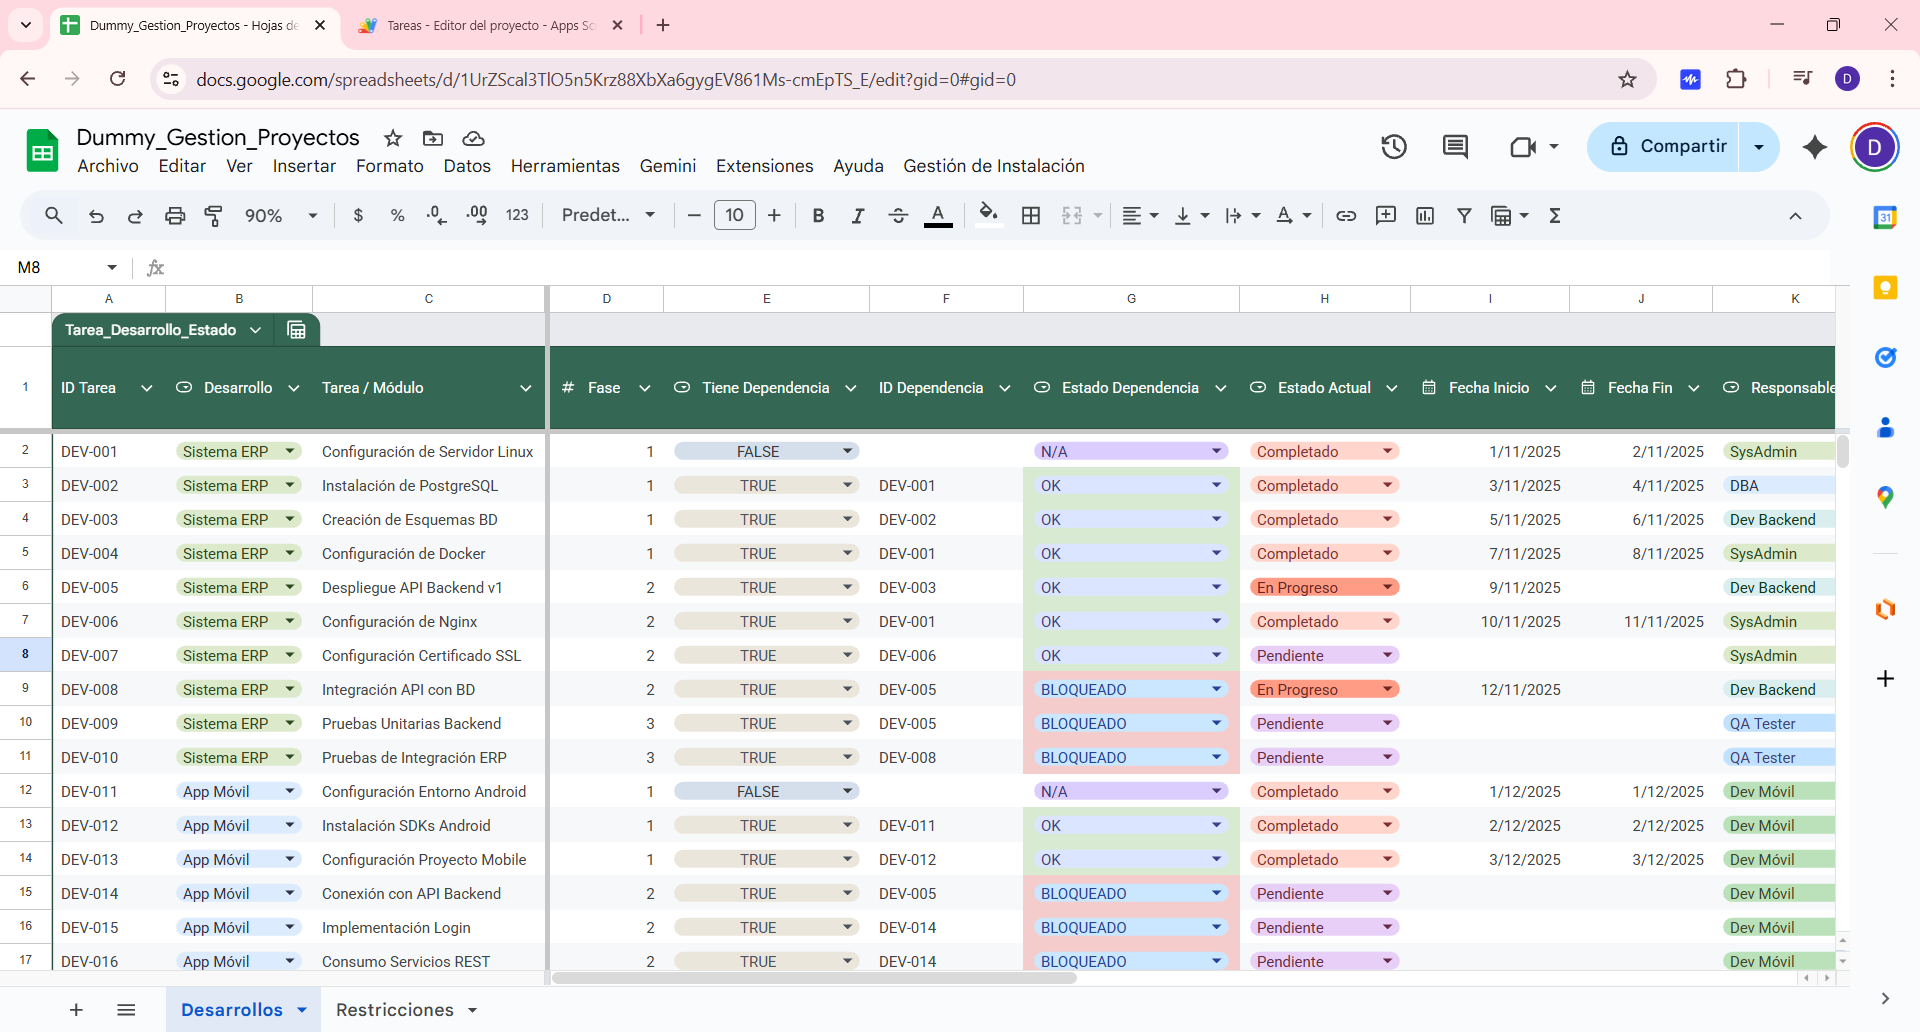
\includegraphics[width=0.95\textwidth]{E6/E6_1.png}
    \caption{Vista general de la hoja de control de tareas operativas con registros ficticios, incluyendo campos de dependencia y estatus, utilizada como base para la automatización del seguimiento.}
\end{figure}

\begin{figure}[H]
    \centering
    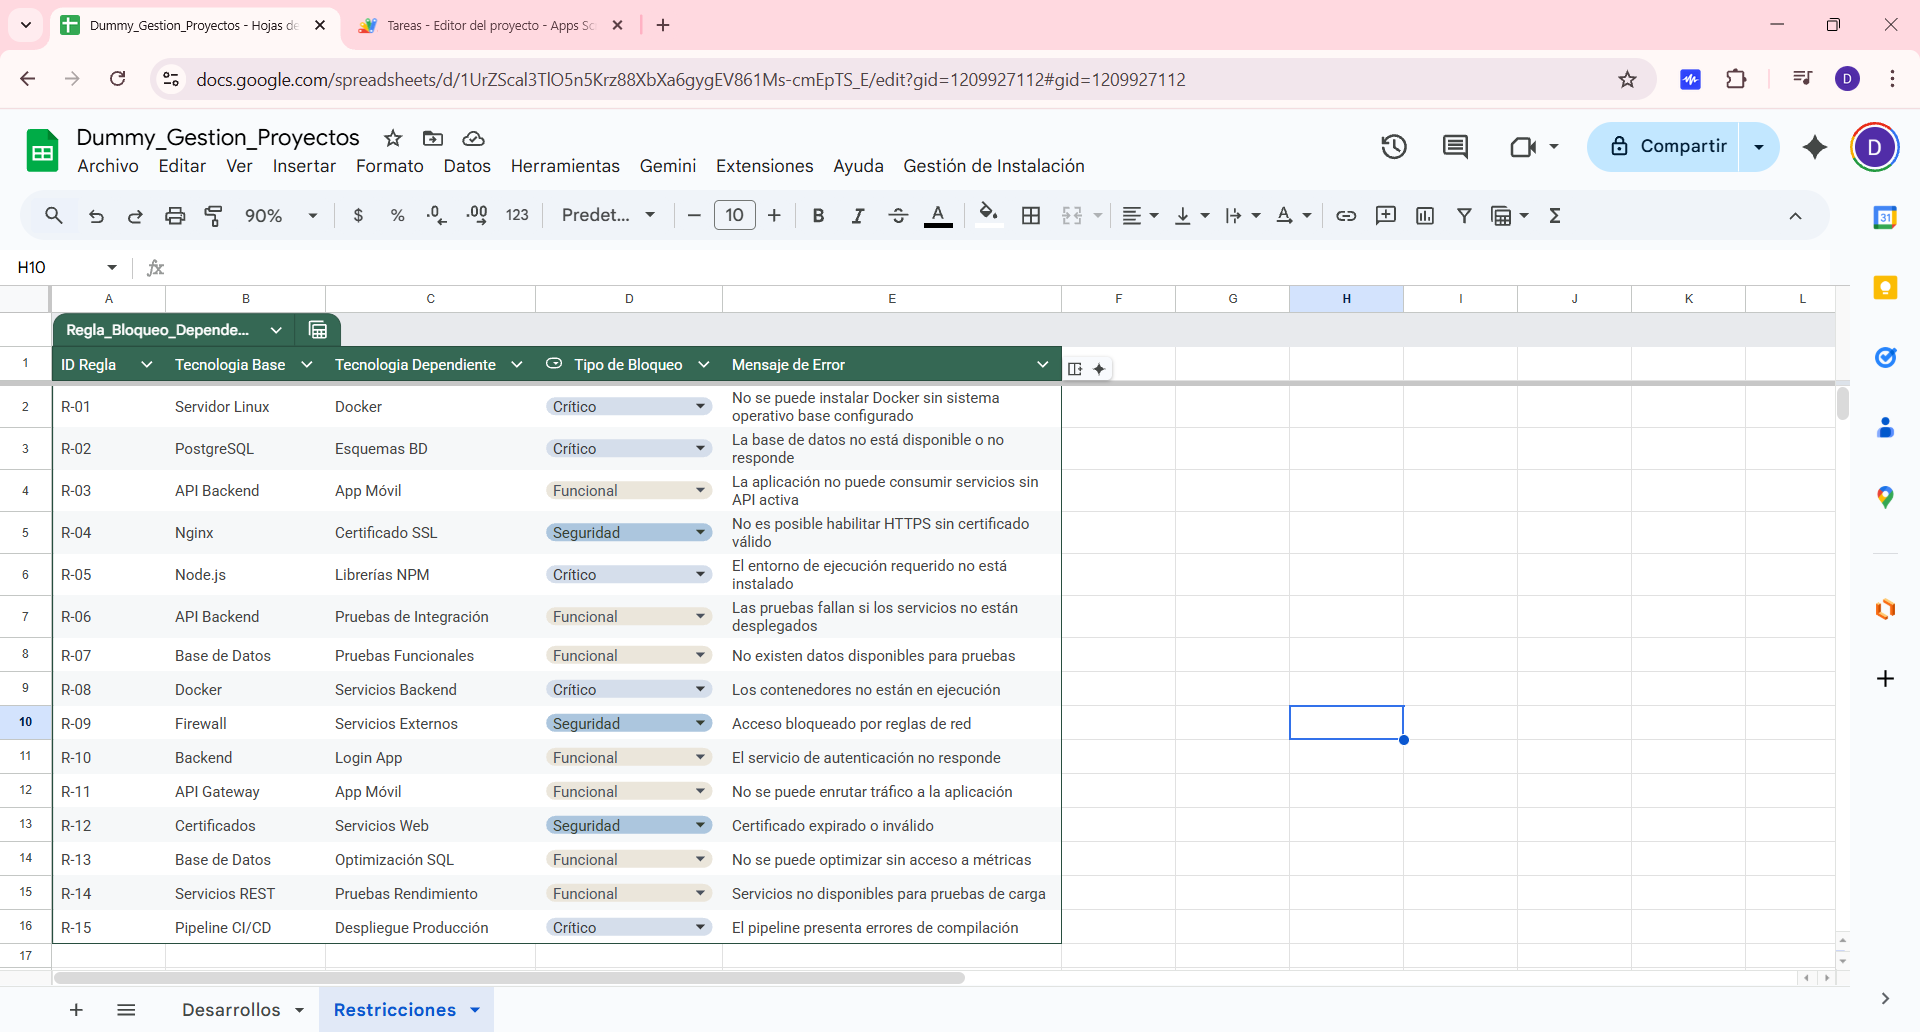
\includegraphics[width=0.95\textwidth]{E6/E6_2.png}
    \caption{Catálogo de reglas y restricciones operativas documentado en una hoja auxiliar, utilizado para estandarizar criterios de bloqueo y validación de dependencias.}
\end{figure}

\begin{figure}[H]
    \centering
    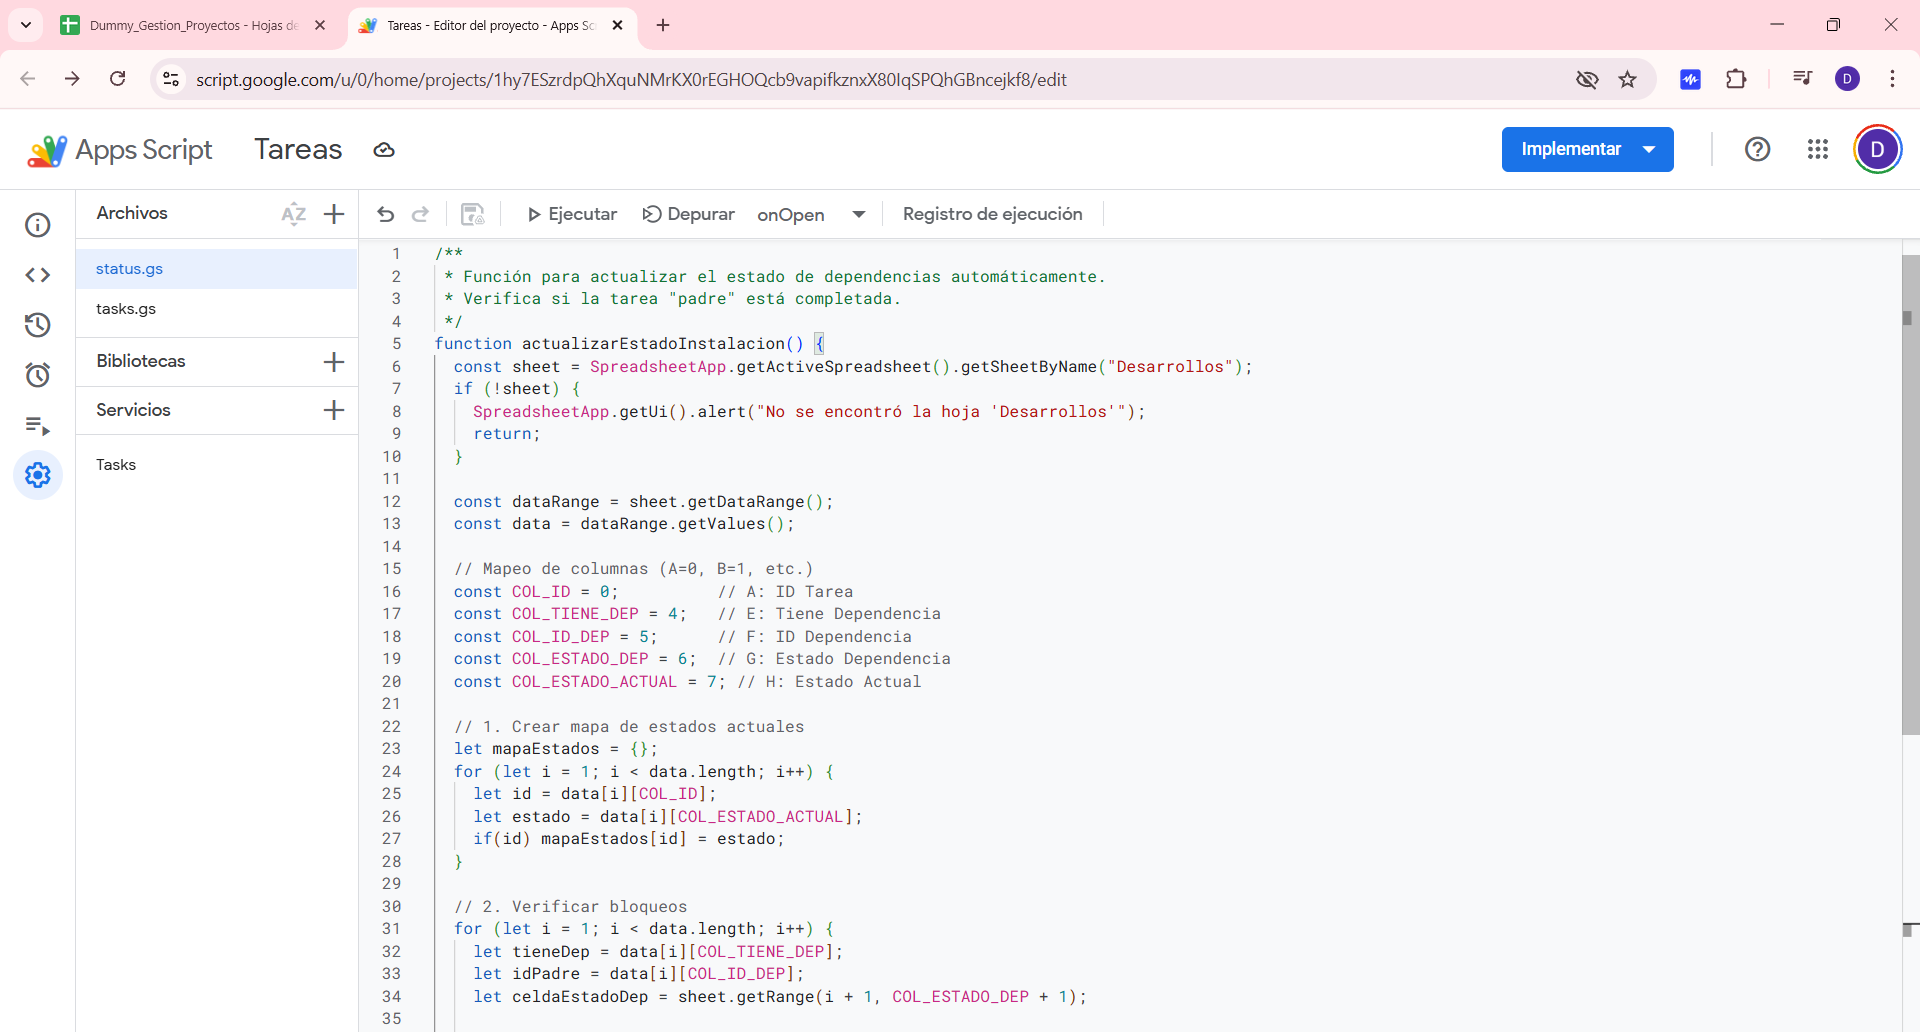
\includegraphics[width=0.95\textwidth]{E6/E6_3.png}
    \caption{Implementación del script de control de dependencias, mostrando la lectura de registros y la construcción de una referencia interna de estatus por identificador.}
\end{figure}

\begin{figure}[H]
    \centering
    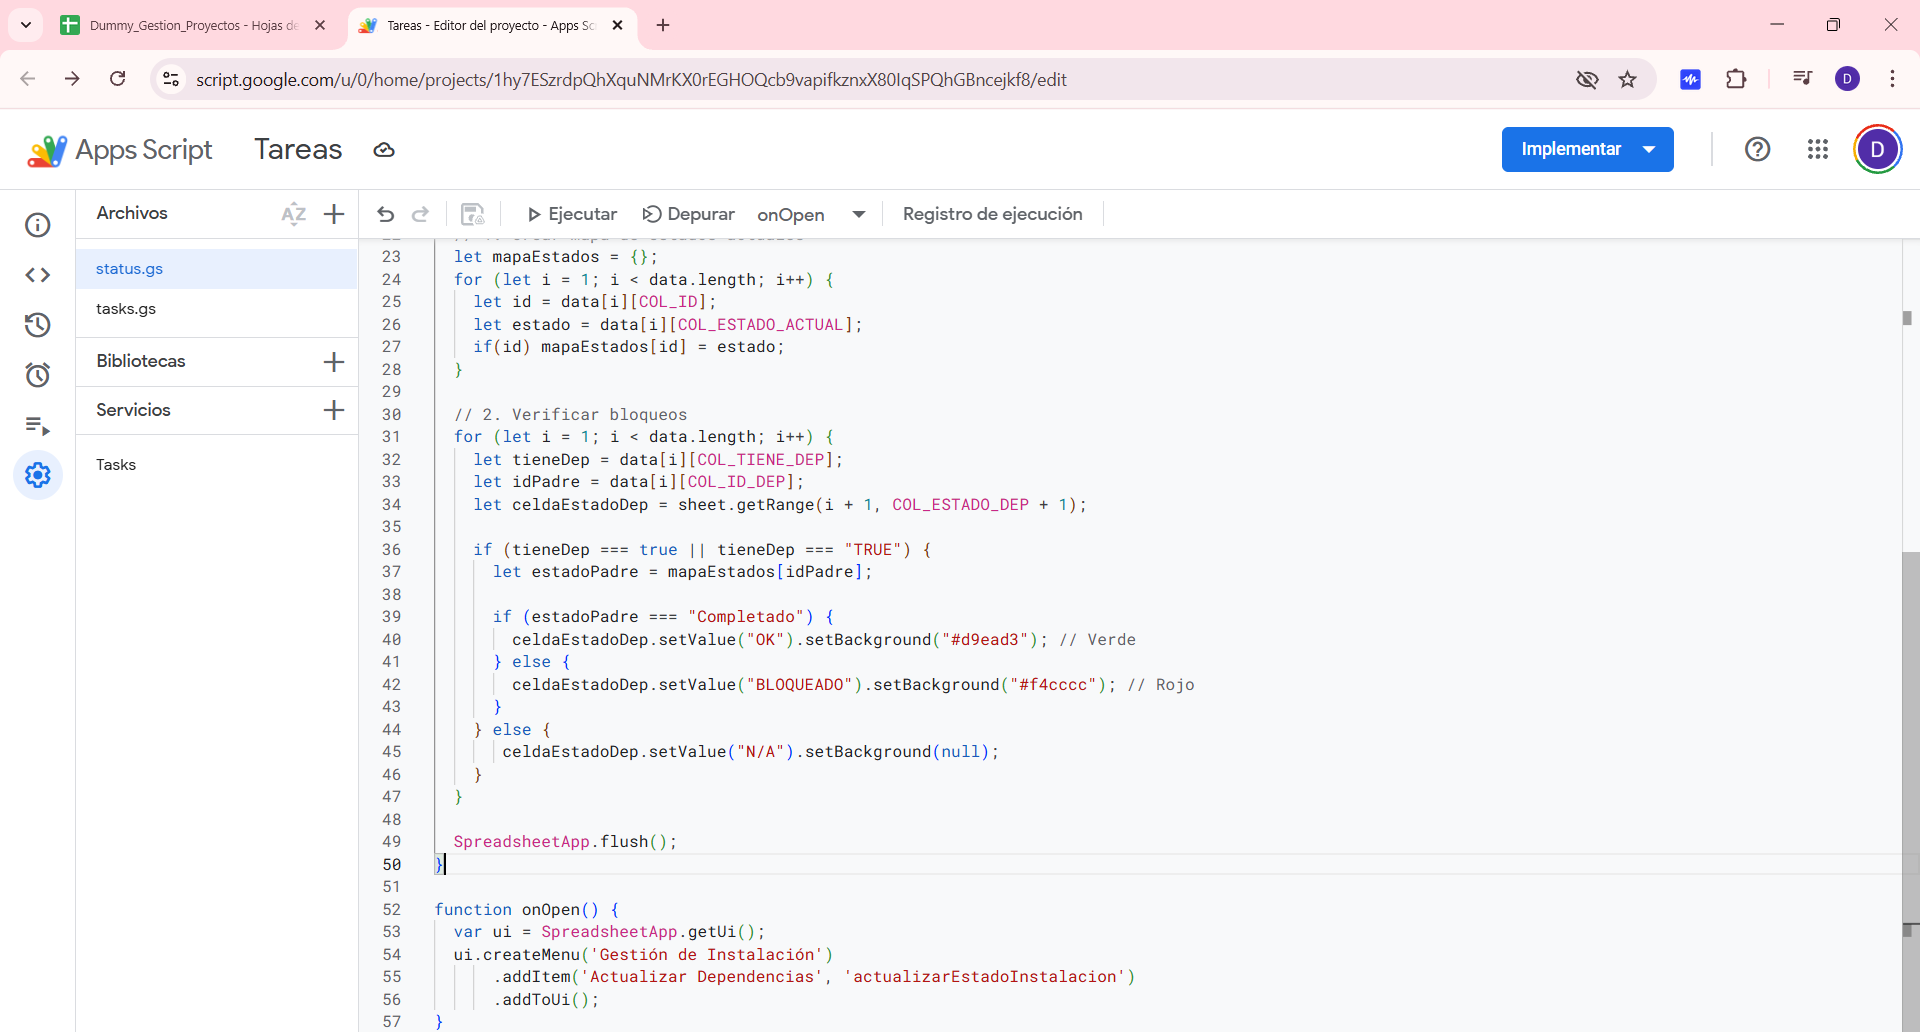
\includegraphics[width=0.95\textwidth]{E6/E6_4.png}
    \caption{Lógica de validación de dependencias y asignación automática de estados, junto con la integración de una opción de menú para la ejecución controlada del script.}
\end{figure}

\begin{figure}[H]
    \centering
    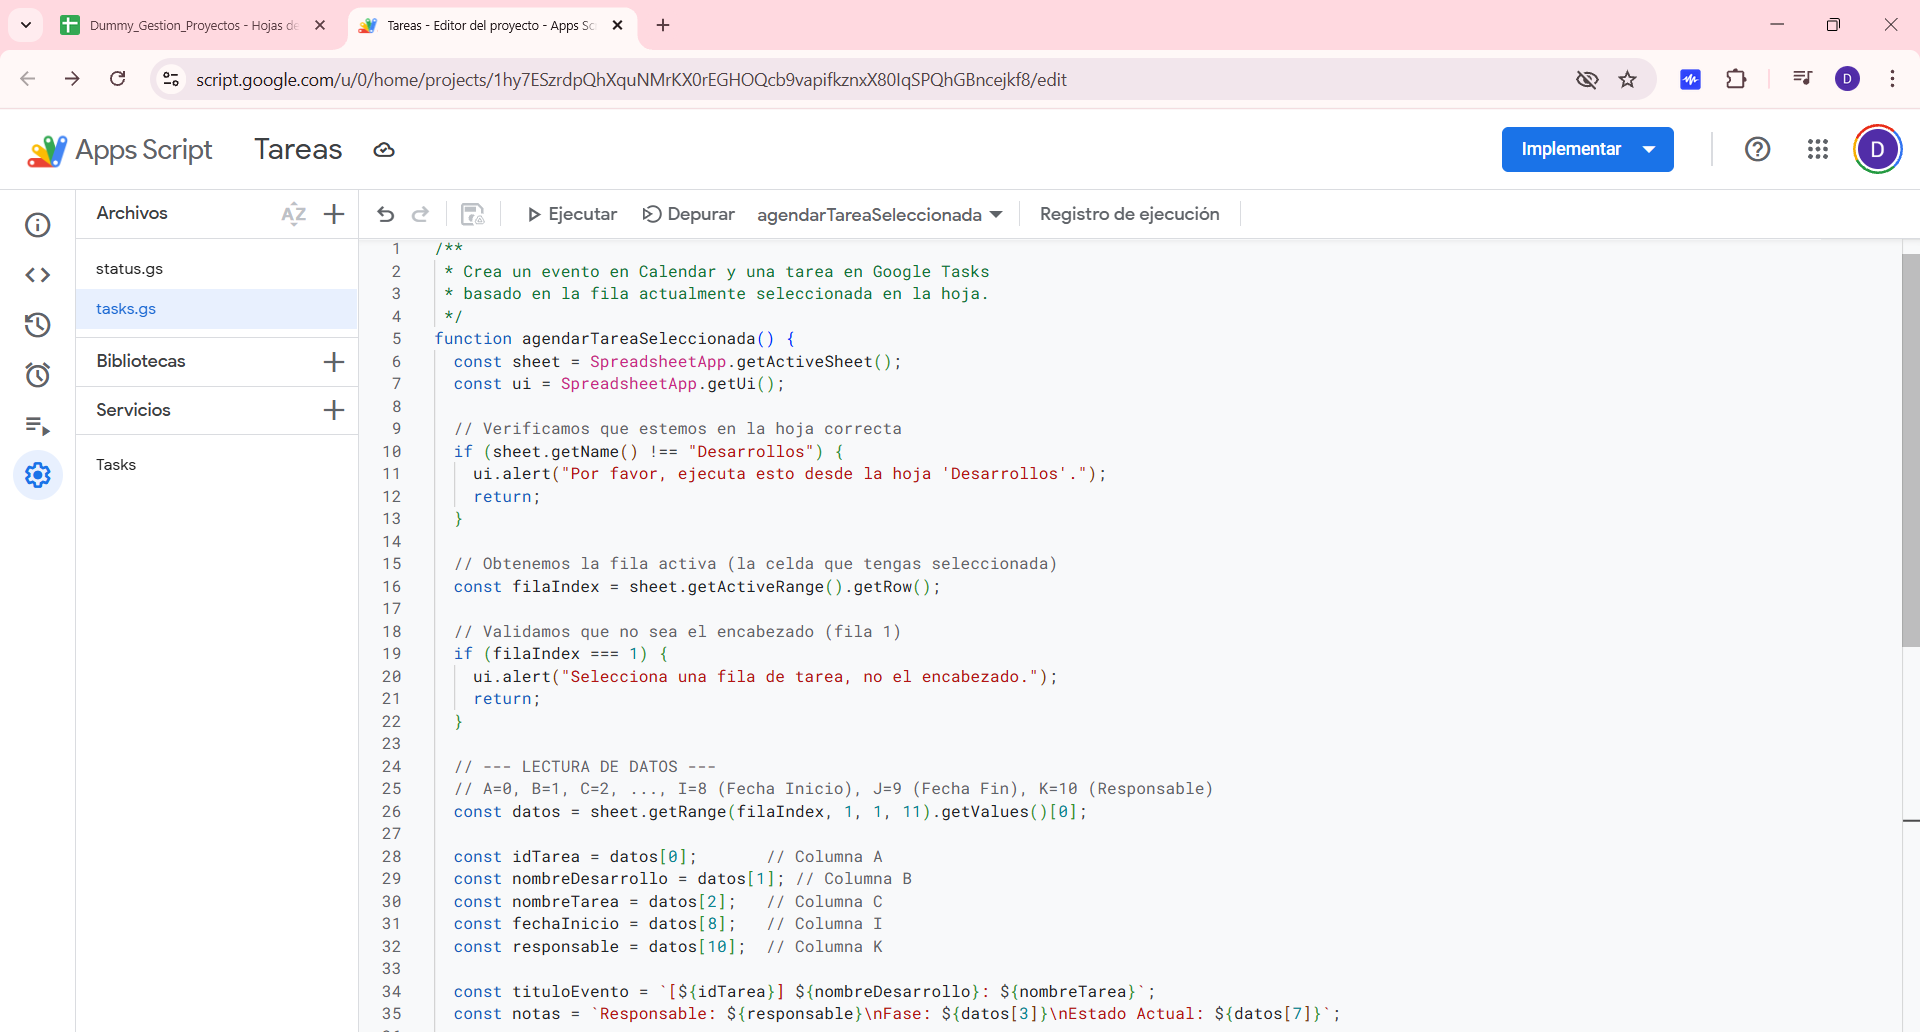
\includegraphics[width=0.95\textwidth]{E6/E6_5.png}
    \caption{Implementación del script de agendamiento automático, mostrando la validación de contexto y la extracción de datos clave desde la fila seleccionada.}
\end{figure}

\begin{figure}[H]
    \centering
    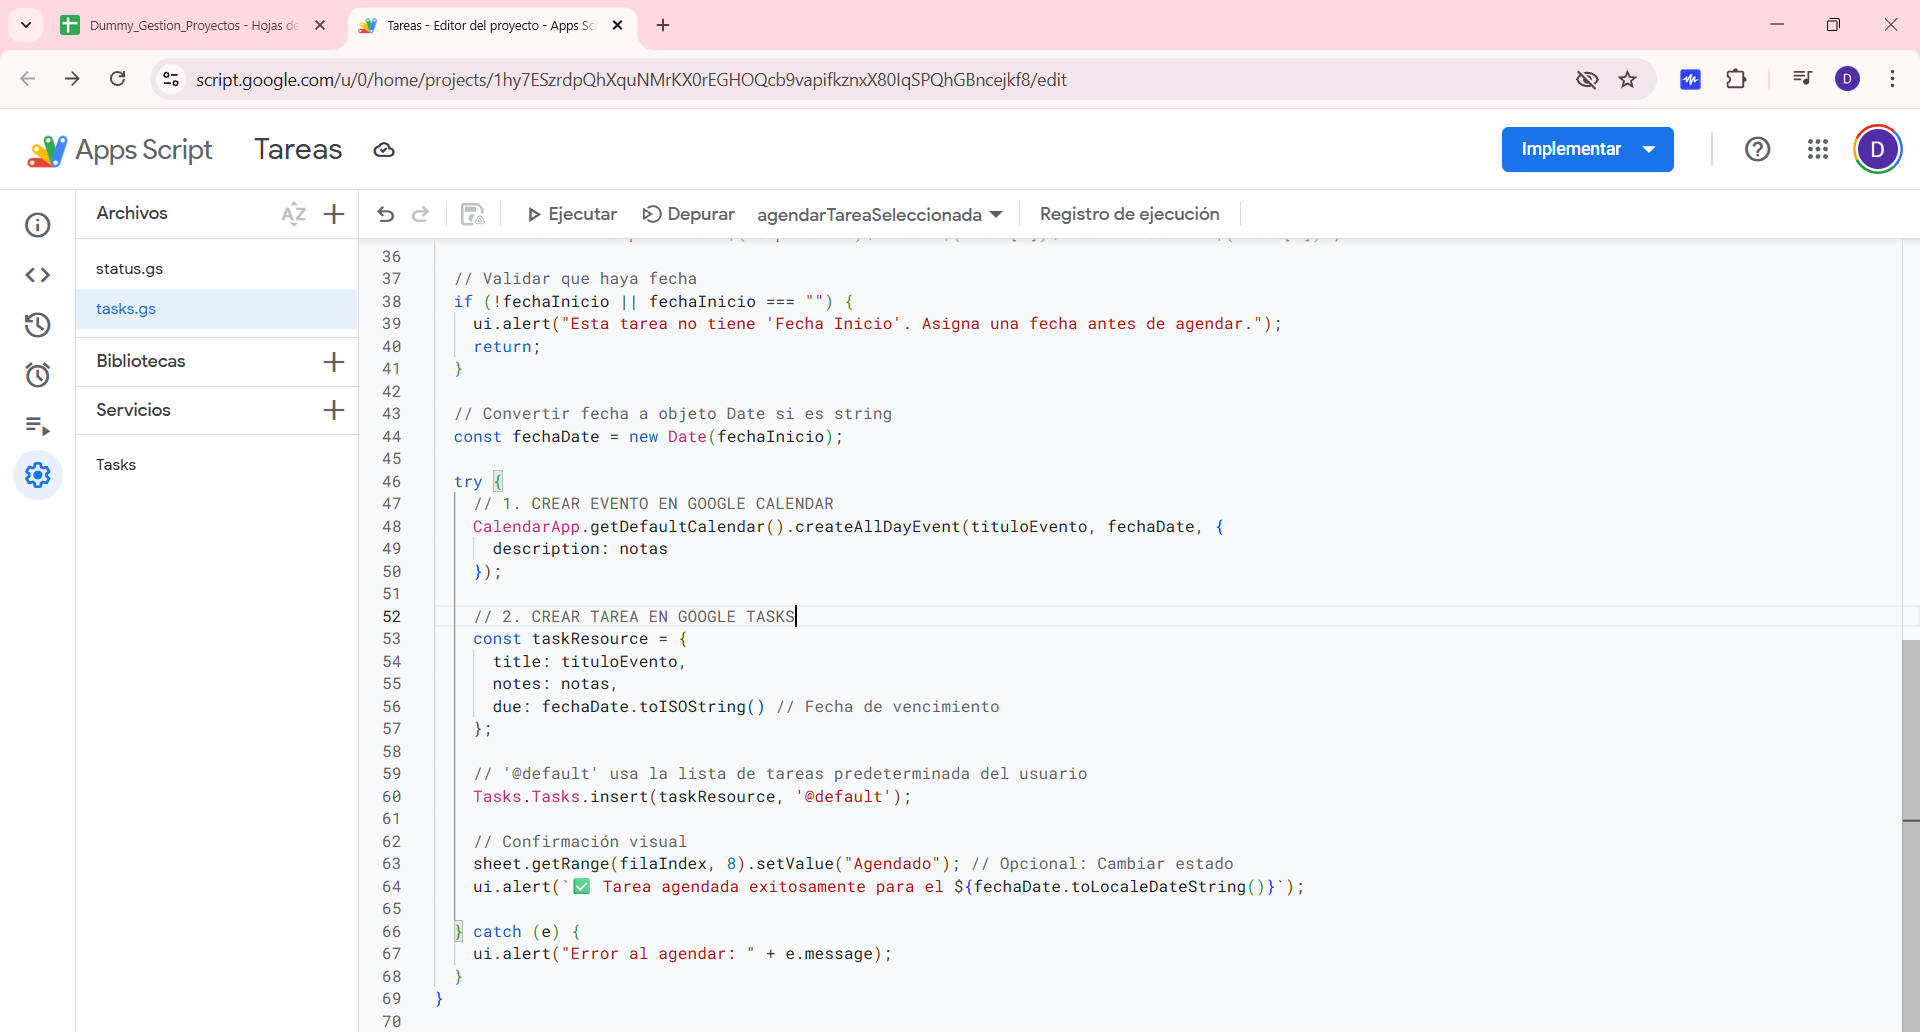
\includegraphics[width=0.95\textwidth]{E6/E6_6.png}
    \caption{Ejecución del proceso de agendamiento automático, incluyendo la creación de eventos y tareas de seguimiento con manejo de excepciones y retroalimentación al usuario.}
\end{figure}

\begin{figure}[H]
    \centering
    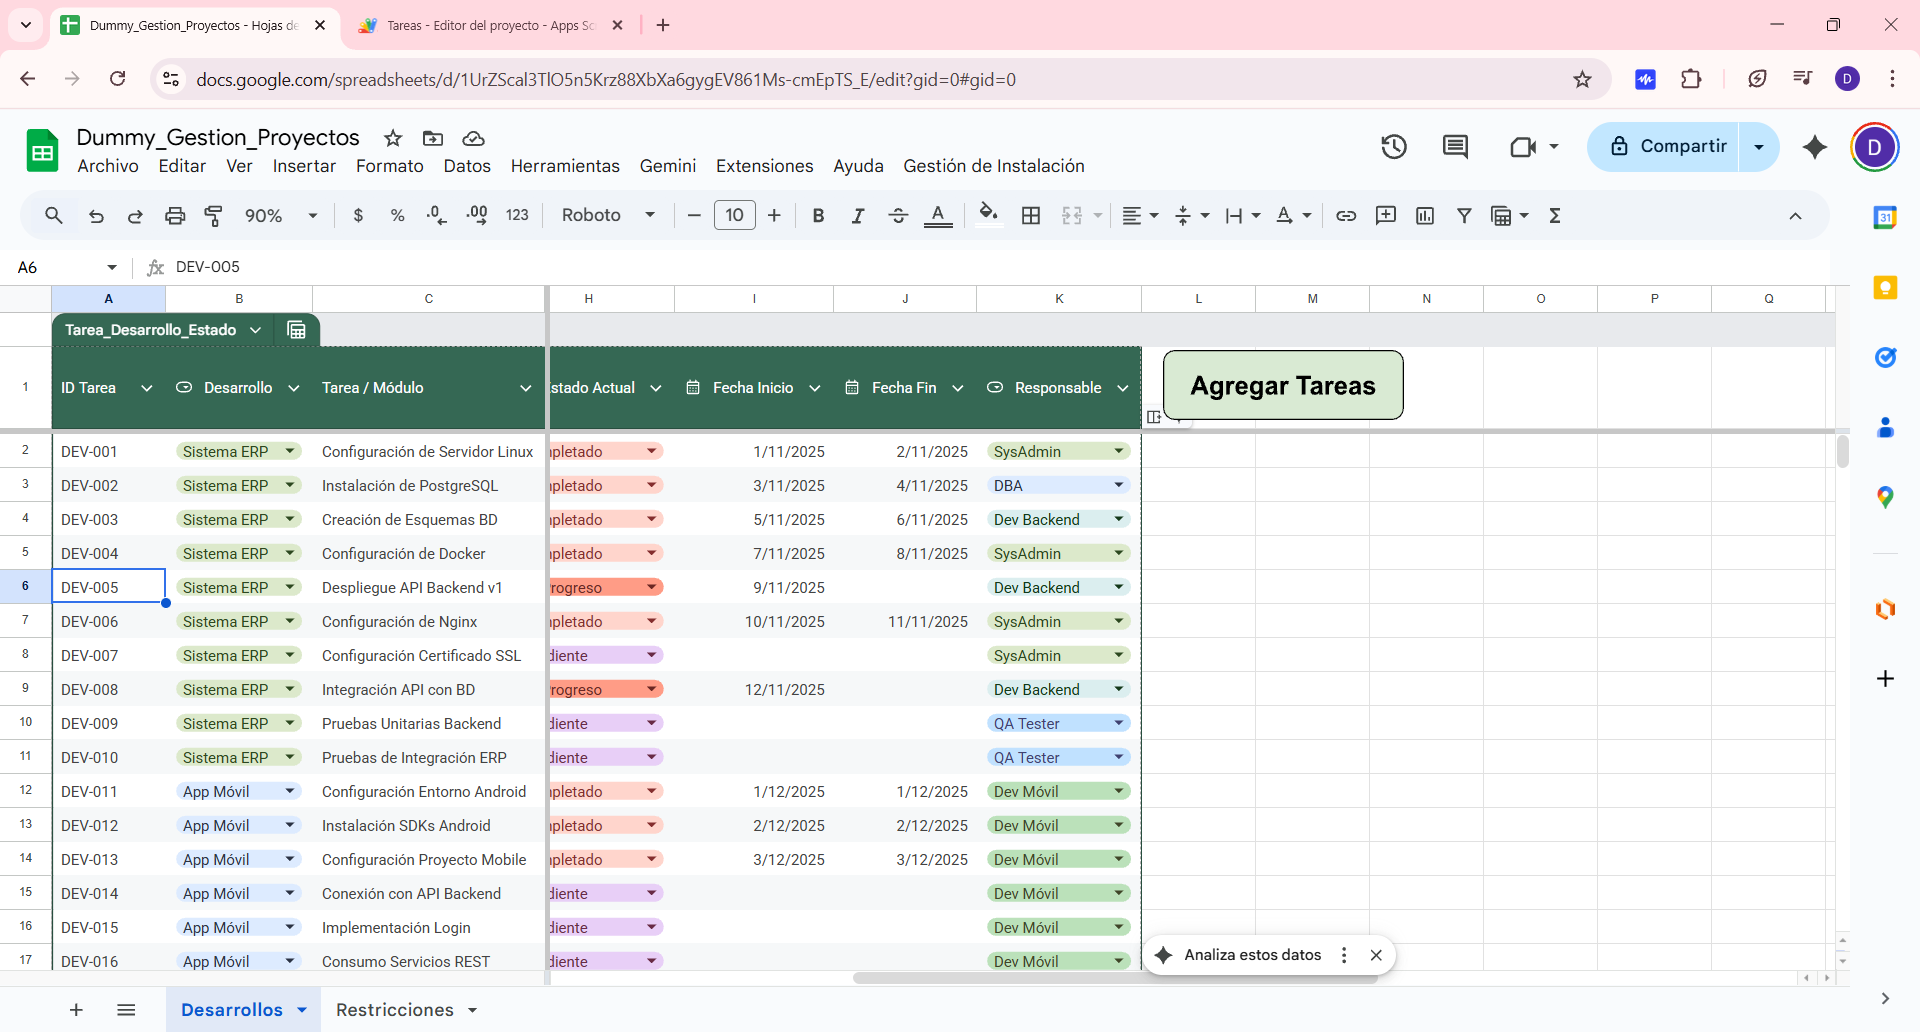
\includegraphics[width=0.95\textwidth]{E6/E6_7.png}
    \caption{Integración de un control de ejecución en la hoja de cálculo mediante un botón de acción para disparar la automatización sobre la tarea seleccionada.}
\end{figure}

\begin{figure}[H]
    \centering
    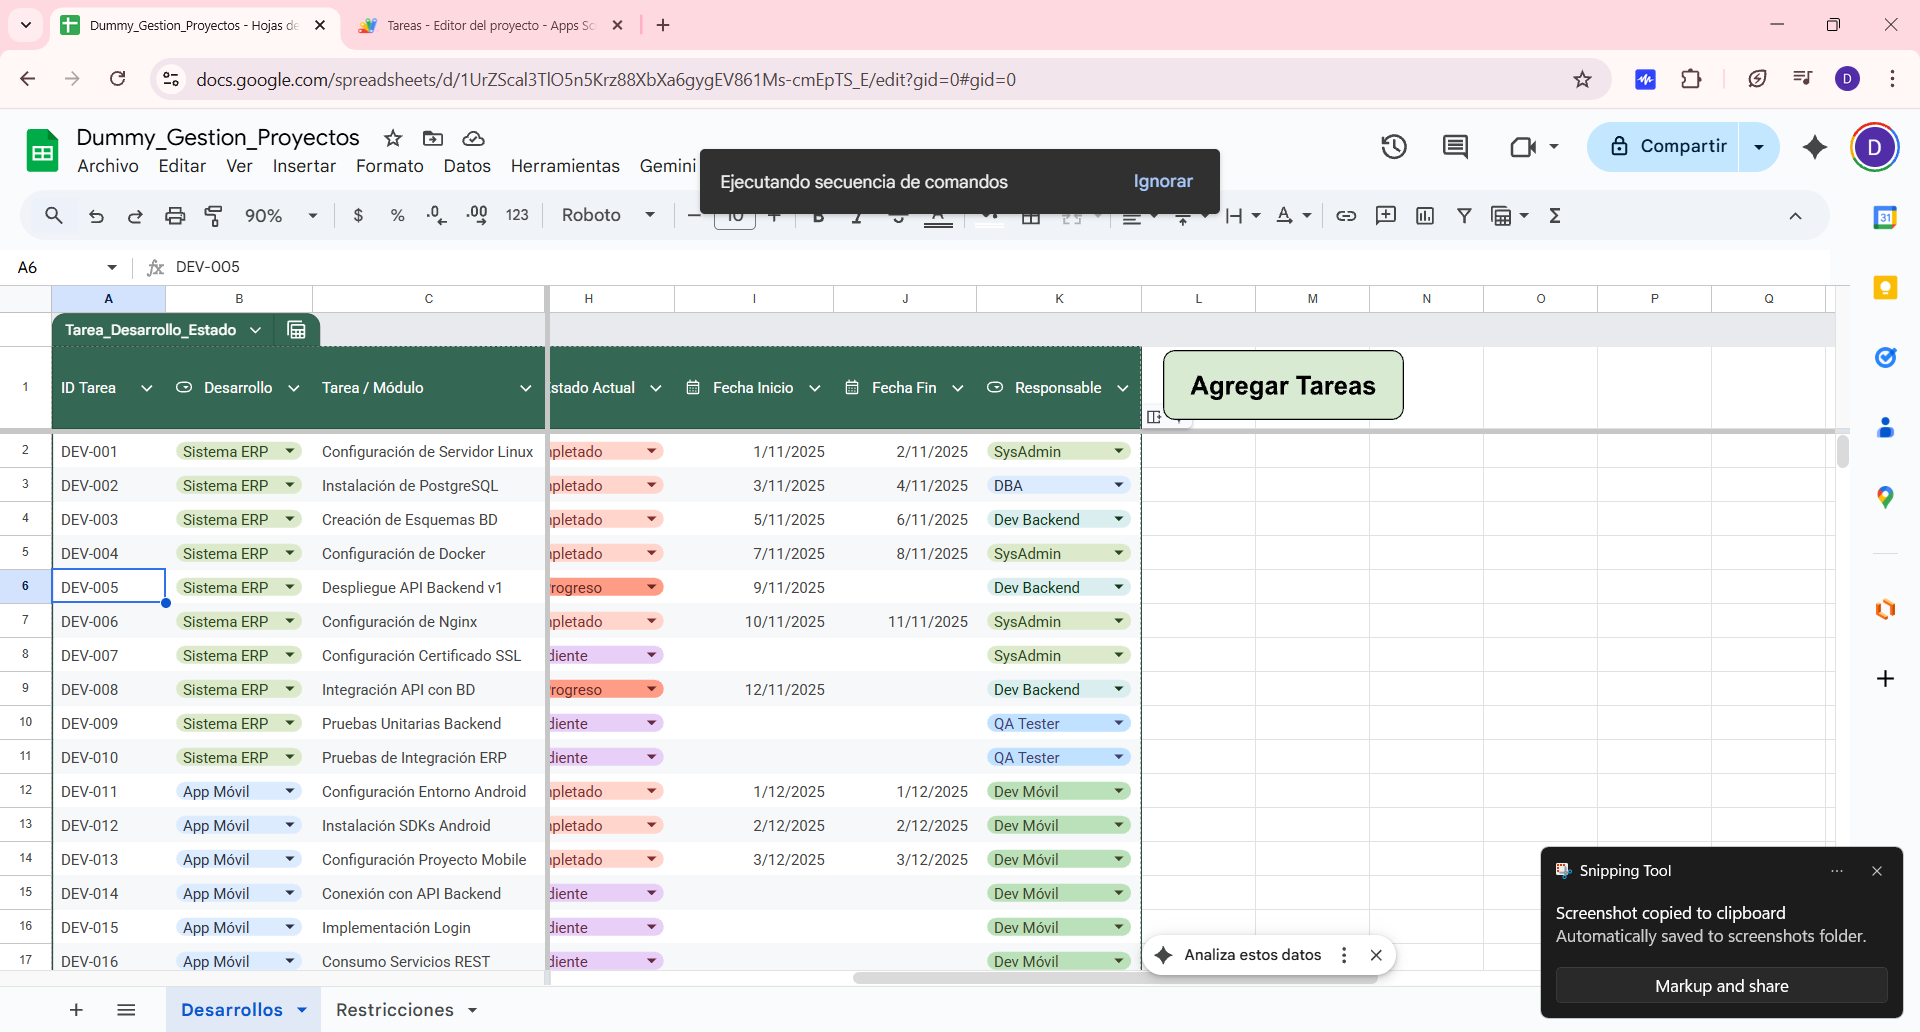
\includegraphics[width=0.95\textwidth]{E6/E6_8.png}
    \caption{Evidencia de la ejecución del script desde la interfaz de usuario, mostrando el flujo de comandos activo durante la operación.}
\end{figure}

\begin{figure}[H]
    \centering
    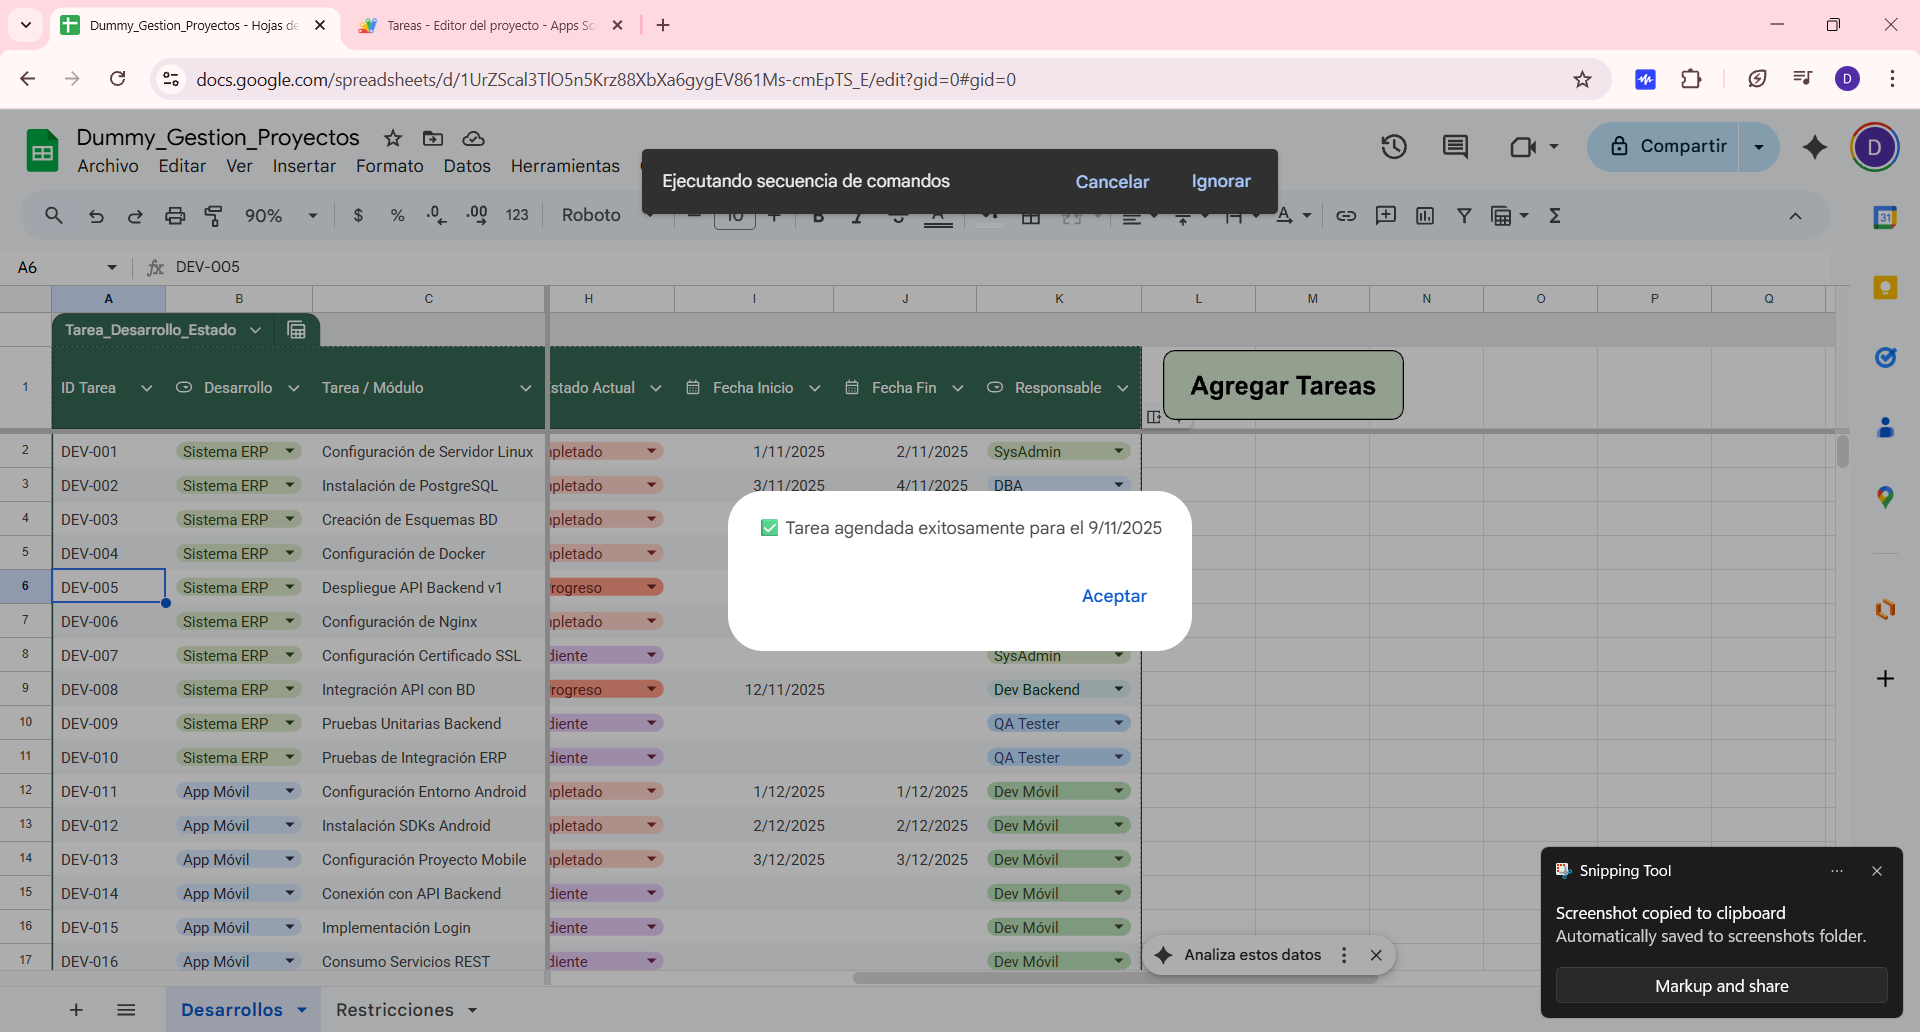
\includegraphics[width=0.95\textwidth]{E6/E6_9.png}
    \caption{Confirmación visual de la ejecución exitosa del proceso automatizado, indicando el correcto agendamiento de la tarea.}
\end{figure}

\begin{figure}[H]
    \centering
    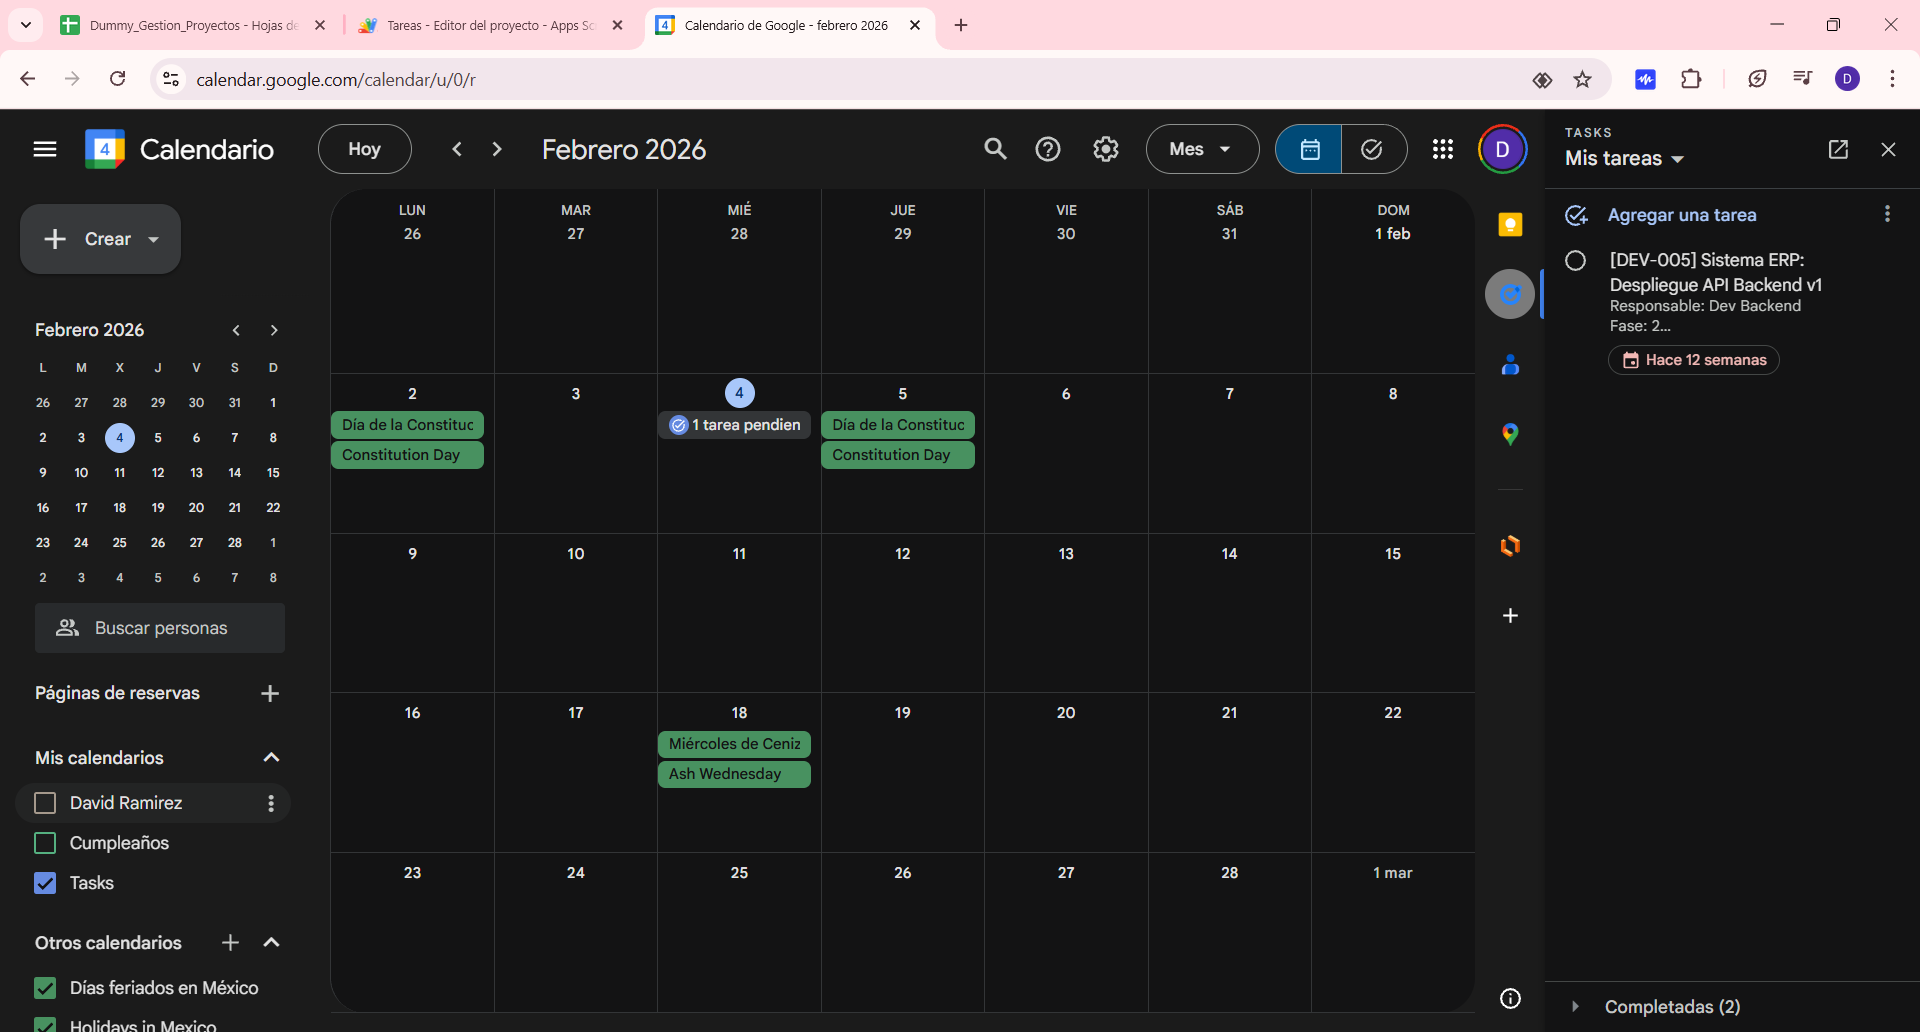
\includegraphics[width=0.95\textwidth]{E6/E6_10.png}
    \caption{Validación del resultado en la herramienta de calendario, mostrando el evento y la tarea generados automáticamente a partir del registro seleccionado.}
\end{figure}


\end{document}

